\documentclass[a4paper,12pt]{article}

%%% Работа с русским языком
\usepackage{cmap}					% поиск в PDF
\usepackage{mathtext} 				% русские буквы в формулах
\usepackage[T2A]{fontenc}			% кодировка
\usepackage[utf8]{inputenc}			% кодировка исходного текста
\usepackage[english,russian]{babel}	% локализация и переносы
\usepackage{xcolor}
\usepackage{hyperref}
 % Цвета для гиперссылок
\definecolor{linkcolor}{HTML}{799B03} % цвет ссылок
\definecolor{urlcolor}{HTML}{799B03} % цвет гиперссылок

\hypersetup{pdfstartview=FitH,  linkcolor=linkcolor,urlcolor=urlcolor, colorlinks=true}

%%% Дополнительная работа с математикой
\usepackage{amsfonts,amssymb,amsthm,mathtools} % AMS
\usepackage{amsmath}
\usepackage{icomma} % "Умная" запятая: $0,2$ --- число, $0, 2$ --- перечисление

%% Номера формул
%\mathtoolsset{showonlyrefs=true} % Показывать номера только у тех формул, на которые есть \eqref{} в тексте.

%% Шрифты
\usepackage{euscript}	 % Шрифт Евклид
\usepackage{mathrsfs} % Красивый матшрифт

%% Свои команды
\DeclareMathOperator{\sgn}{\mathop{sgn}}

%% Перенос знаков в формулах (по Львовскому)
\newcommand*{\hm}[1]{#1\nobreak\discretionary{}
{\hbox{$\mathsurround=0pt #1$}}{}}
% графика
\usepackage{graphicx}
\graphicspath{{pictures/}}
\DeclareGraphicsExtensions{.pdf,.png,.jpg}
\author{Бурмашев Григорий, БПМИ-208}
\title{NIS22DSP, Контрольная работа, вариант 3}
\date{\today}
\begin{document}
\maketitle

\section*{Задача 1}
\begin{center}

\includegraphics[scale=0.4]{1.png}
\end{center}
\[
x[n] = e^{j \pi \frac{n}{11}}
\]
\[
x[n] = x[n + N] = e^{\frac{i \pi (n + N)}{11}} = 
e^{\frac{i \pi n}{11}} \cdot e^{\frac{i \pi N}{11}}
\]
Проверим, равен ли правый знаменатель единице:
\[
e^{\frac{i \pi N}{11}} = 1
\]
\[
\frac{\pi N }{11} = 2 \pi k
\]
\[
\frac{N}{11} = 2 k
\]
\[
N = 22k, \; k \in \mathbb{Z}
\]
При $k = 1$ получаем $N = 22$
\begin{center}
\textbf{Ответ: } 
\[
x[n] - \text{периодический сигнал с периодом } N = 22
\]
\end{center}
\clearpage
\section*{Номер 2}
\begin{center}

\includegraphics[scale=0.4]{2.png}
\end{center}
\[
h[n] = 2^n u [-n - 3]
\]
\[
x[n] = u[n - 8]
\]
\[
y[n] = \sum_{k = -\infty}^{\infty } h[k] \cdot x[n - k]  = 
\]
\[
=
\sum_{k = -\infty}^{\infty }  
2^k u[-k - 3] \cdot u[n - k - 8]
\]
\begin{enumerate}
\item
\[
u[-k - 3] = 
\begin{cases}
1, k \leq -3 \\
0, k > -3
\end{cases}
\]
\item
\[
u[n - k - 8 ] = 
\begin{cases}
1, k  \leq n - 8 \\
0, k > n - 8
\end{cases}
\]
\end{enumerate}
Тогда по геометрической прогрессии получаем:
\[
\sum_{k=-\infty}^{n - 8} 2^k = 2^{n - 7}
\]
\[
\sum_{k=-\infty}^{-3} 2^k = \frac{1}{4}
\] 
\begin{center}
\textbf{Ответ: } 
\[
\sum_{k=-\infty}^{n - 8} 2^k = 2^{n - 7}
\]
\[
\sum_{k=-\infty}^{-3} 2^k = \frac{1}{4}
\] 
\end{center}
\clearpage
\section*{Номер 3}
\begin{center}
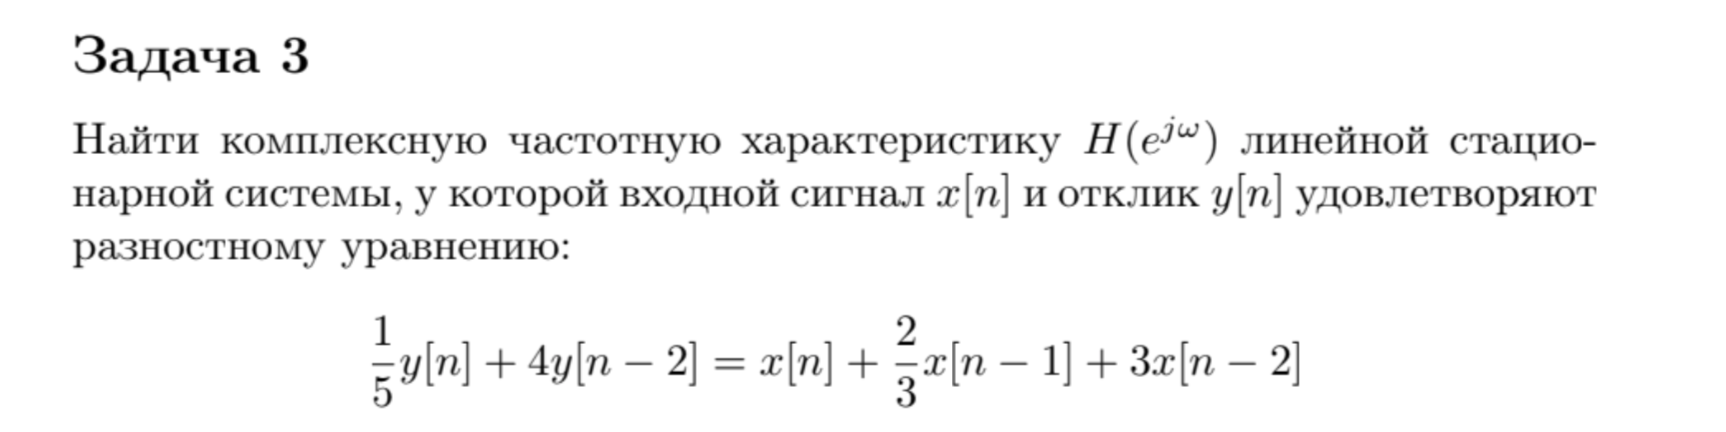
\includegraphics[scale=0.4]{3.png}
\end{center}
\[
\frac15 y[n] + 4y[n-2] = x[n] + \frac23 x[n-1] + 3x[n-2]
\]
Знаем, что:
\[
H(e^{jw}) = \mathcal{F} \left( h[k] \right) = \sum_{k = -\infty}^{+\infty} h[k] e^{-i \omega k}
\]
\[
h[k] = \mathcal{S} (\delta [k])
\]
Проверяем:
\[
\frac15 h[n] + 4h[n-2] = \delta[n] + \frac23 \delta[n-1] + 3\delta[n-2]
\]
\[
\frac15 H(\omega) + 4 H(\omega) \cdot e^{-i \omega 2}
=
3 \cdot 1 + \frac23 \cdot 1 \cdot e^{-i \omega 1} + 3 \cdot 1 \cdot e^{-i \omega 2}
\]
\[
\frac15 H(\omega) + 4 H(\omega) \cdot e^{-i \omega 2} = 3 + \frac{2}{3} \cdot e^{- i \omega} + 3 \cdot e^{-i \omega 2}
\]
\[
H(\omega) + 20H(\omega) \cdot e^{-i \omega 2} = 15 + \frac{10}{3} \cdot e^{- i \omega} + 15 \cdot e^{-i \omega 2}
\]
\[
H(\omega) \cdot (1 + 20 e^{-i\omega2}) = 15 + \frac{10}{3} \cdot e^{- i \omega} + 15 \cdot e^{-i \omega 2}
\]
\[
H(\omega) = \frac{15 + \frac{10}{3} \cdot e^{- i \omega} + 15 \cdot e^{-i \omega 2}}{1 + 20 e^{-i\omega2}}
\]
\begin{center}
\textbf{Ответ: } 
\[
H(\omega) = \frac{15 + \frac{10}{3} \cdot e^{- i \omega} + 15 \cdot e^{-i \omega 2}}{1 + 20 e^{-i\omega2}}
\]
\end{center}
\clearpage
\section*{Номер 4}
\begin{center}
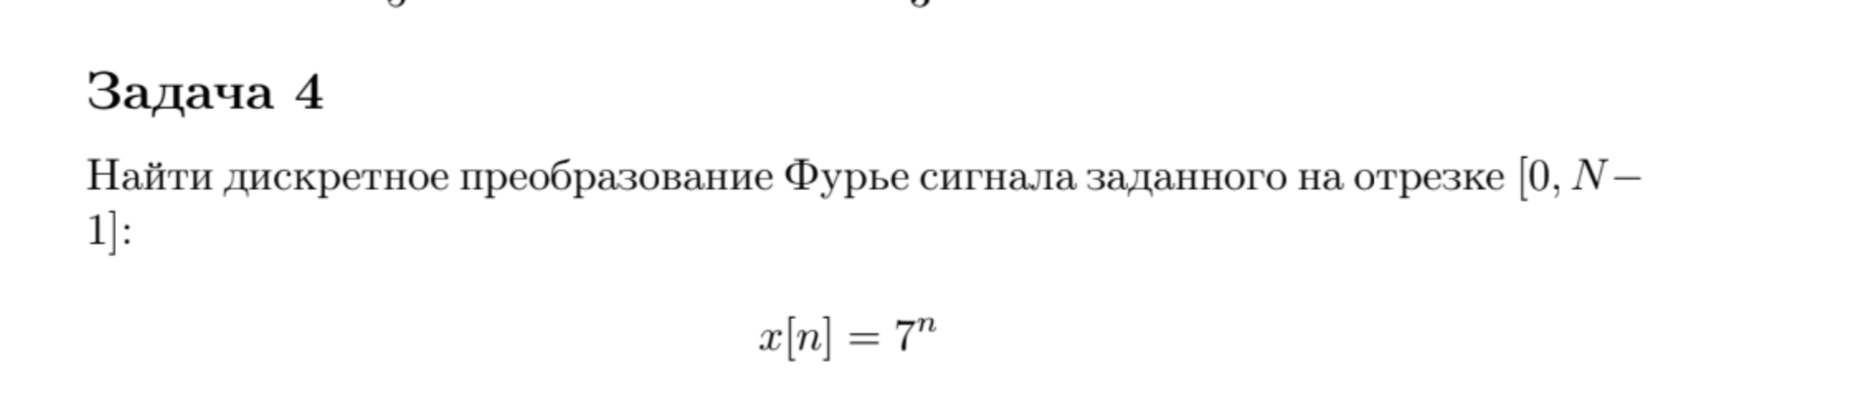
\includegraphics[scale=0.4]{4.png}
\end{center}
\[
x[n] = 7^n
\]
Применяем формулу:
\[
X[k] = \sum_{n = 0}^{N - 1} x[n] e^{-i n \omega_k}
\]
\[
X[k] = \sum_{n = 0}^{N - 1} 7^n e^{-i n \frac{2 \pi k}{N}} =
\sum_{n = 0}^{N - 1}
\left(
7 e^{-i \frac{2 \pi k}{N}}
\right)^n
=
\frac{1 - \left( 7 e^{-i \frac{2 \pi k}{N}} \right)^N}{1 - 7 e^{-i \frac{2 \pi k}{N}}} =
\]
\[
=
\frac{1 - 7^N e^{-i 2 \pi k}}{1 - 7 e^{-i \frac{2 \pi k}{N}}}  =
\frac{1 - 7^N}{1 - 7 e^{-i \frac{2 \pi k}{N}}}
\]
\begin{center}
\textbf{Ответ: } 
\[
\frac{1 - 7^N}{1 - 7 e^{-i \frac{2 \pi k}{N}}}
\]
\end{center}
\end{document}
